\subsubsection{子集}

我们知道,任何一个自然数都是一个整数,就是说,自然数集$N$的任何一个元素都是整数集$Z$的一个元素。同样,自然数集$N$的任何一个元素都是有理数集$Q$的一个元素。

对于两个集合$A$与$B$,如果集合$A$的任何一个元素都是集合$B$的元素,那么集合$A$叫做集合$B$的\textbf{子集},记作
$$A \subseteq B \quad \text{(或} B \supseteq A \text{),}$$
读作“$A$包含于$B$”(或“$B$包含$A$”)。例如
$$N \subseteq Z, \quad N \subseteq Q, \quad R \supseteq Z, \quad R \supseteq Q \text{。}$$

当$A$不是$B$的子集时,我们可以记作
$$A \not \subseteq B \quad \text{(或} B \not \supseteq A \text{),}$$
读作“$A$不包含于$B$”(或“$B$不包含$A$”)。

对于任何一个集合$A$,因为它的任何一个元素都属于集合$A$本身,所以
$$A \subseteq A \text{,}$$
也就是说,\textbf{任何一个集合是它本身的子集}。

为了方便起见,我们把不含任何元素的集合叫做\textbf{空集},记作$\kongji$。例如:
\begin{gather*} 
    \{x \mid x+1=x+3\} = \kongji \ \text{,} \\
    \{\text{小于零的正整数}\} = \kongji \ \text{,} \\
    \{\text{两边之和小于第三边的三角形}\} = \kongji \ \text{。}
\end{gather*}

我们规定\textbf{空集是任何集合的子集}。也就是说,对于任何集合$A$,有
$$\kongji \subseteq A \quad \text{。}$$

如果$A$是$B$的子集,并且$B$中至少有一个元素不属于$A$,那么集合$A$叫做集合$B$的\textbf{真子集},记作
$$A \subset B \quad \text{(或} B \supset A \text{)。}$$

当$A$不是$B$的真子集时,我们可以记作
$$A \not \subset B \quad \text{(或} B \not \supset A \text{)。}$$

例如,自然数集$N$是$N$的子集,但不是的$N$真子集,所以$N \subseteq N$,但 $N \not \subset N$;$N$是实数集$R$的子集,也是$R$的真子集,所以$N \subset R$。

\begin{wrapfigure}[10]{r}{4.5cm}
    \centering
    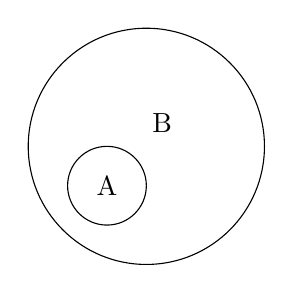
\begin{tikzpicture}
        \draw (2.5,0.5) circle [radius=0.5];
        \node at (2.5, 0.5) {A};
        \draw (3.0,1.0) circle [radius=1.5];
        \node at (3.2, 1.3) {B};
    \end{tikzpicture}
    \vspace{-10pt}
    \caption{}\label{fig:1-1}
\end{wrapfigure}

集合$B$同它的真子集$A$之间的关系,可以用 图\ref{fig:1-1} 中$B$同$A$的关系来说明,其中$A$,$B$两个圈的内部分别表示集合$A$,$B$。

显然,空集是任何非空集合的真子集。

容易知道,\textbf{对于集合$A$,$B$,$C$,如果$A \subseteq B$,$B \subseteq C$,那么$A \subseteq C$。}事实上,设 $x$ 是集合$A$的任意一个元素,因为$A \subseteq B$,所以$x \in B$,又因为$B \subseteq C$,所以$x \in C$。从而 $A \subseteq C$。

同样可知,\textbf{对于集合$A$,$B$,$C$,如果$A \subset B$,$B \subset C$,那么$A \subset C$.}

对于两个集合$A$与$B$,如果$A \subseteq B$,同时$B \subseteq A$,我们就说这两个\textbf{集合相等},记作
$$A = B \text{,}$$
读作“$A$等于$B$”。

例如,$A = \{x \mid x^2+3x+2=0\}$,$B = \{-1, -2\}$,则 $$A = B \text{。}$$

\liti 写出集合$\{a, b\}$的所有子集及真子集。

\jie 集合$\{a, b\}$的所有的子集是$\kongji$,$\{a\}$,$\{b\}$,$\{a,b\}$,其中$\kongji$,$\{a\}$,$\{b\}$是真子集。

\liti 写出不等式 $x-3>2$的解集并进行化简(即化成直接表明未知数本身的取值范围的解集)。

\jie 不等式 $x-3>2$ 的解集是 $$\{x \mid x-3>2\} = \{x \mid x>5\} \text{。}$$
